%priprava posamezne ure
%tukaj zaporedoma napisemo{st. zaporedne ure}{datum}{naslov}{poglavje}{oblika dela}{pripomocki}
\begin{priprava}{}{}{Integral}{Ploščina med dvema funkcijama}{frontalna}{tabla}

\didopomba{Slikca pozitivnih funkcij, iz katere je očitno, da moraš izračunati presečišči in je ploščina enaka razliki ploščin, torej razlika integralov oz. integral razlike.}

\begin{figure}[h]
    \centering
    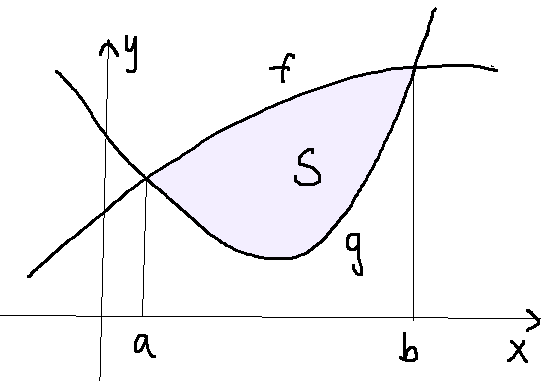
\includegraphics[width=0.4\textwidth]{slike/ploscina_med_dvema.png}
\end{figure}


Izračun ploščine med dvema funkcijama:
\begin{enumerate}
    \item izračunamo presečišča \didopomba{dovolj je $ x $-koordinate} $ \rightarrow a $ in $ b $
    \item $ S = \int_a^b (f(x) - g(x)) dx $ \didopomba{zgornja $ - $ spodnja}
\end{enumerate}

\didopomba{Še ena slika, kjer spodnja funkcija gre pod $ x $-os, premislek, da se pri odštevanju integrala $ g $ tisti negativni del v bistvu prišete k ploščini in dobimo pravi $ S \rightarrow $ formula velja v vseh primerih.}

\begin{figure}[h]
    \centering
    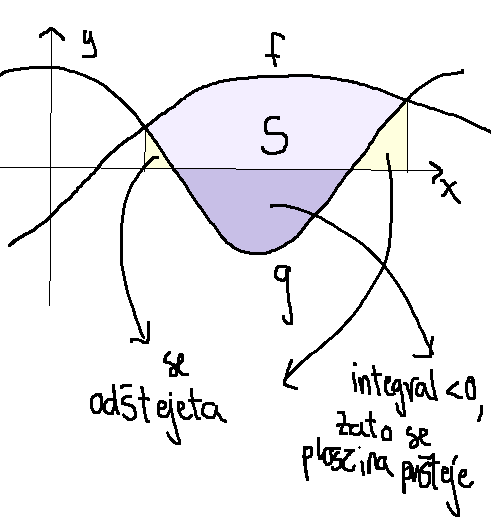
\includegraphics[width=0.4\textwidth]{slike/ploscina_med_dvema_neg.png}
\end{figure}

\didopomba{ALI pa v bistvu samo obe funkciji premakneš za isto navzgor, npr. namesto $ g $ in $ f $ vzameš $ g + 10 $ in $ f + 10 $, da je območje nad $ x $-osjo (in območje se pri premiku ne spremeni) in formula velja, tiste 10-ke pa proč odpadejo in smo na istem.}

\vaje{
Vaje:
\begin{itemize}
    \item Ploščine funkcij, ki jih grafi oklepajo z $ x $-, $ y $-osjo in drugimi premicami ipd., ploščina med funckijama in eno osjo ...
\end{itemize}
}
        
\end{priprava}